\markright{Android Internals}
\section{Android Internals - Overview}
\label{overview}
As we can see in Fig. \ref{fig:stack} \cite{remixingand}, Android's architecture can be divided into many components, which we'll briefly analyse - following a bottom-up approach - before going deeper into the core of this work.
\begin{figure}[!htb]
	\centering
	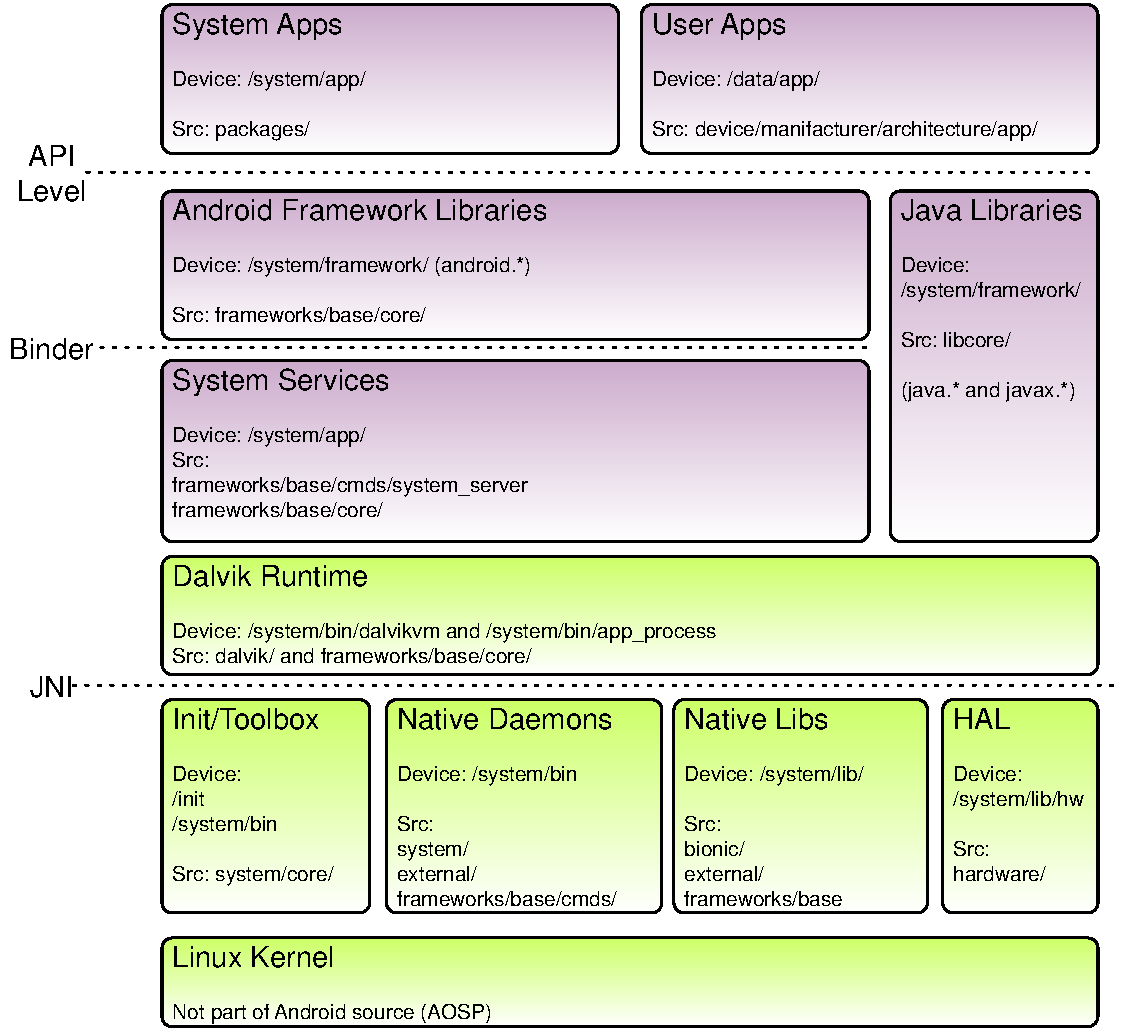
\includegraphics[scale=.6]{images/stack.pdf}
	\caption{Android's stack}
	\label{fig:stack}
\end{figure}
\begin{itemize}
\item \textbf{Linux Kernel}\\
Android kernels are, in sum, forks from the mainline kernel, relying on several custom 	functionalities that are significantly different from what is found in the "vanilla" kernel. Follows a brief enumeration of the most remarkable customizations made to the kernel to satisfy special Android's needs.
	\begin{itemize}
	\item \textsc{Wakelocks}\\
	Instead of letting the system be put to sleep at the user's behest, an "Androidized"
kernel is made to go to sleep as soon and as often as possible. \textit{Wakelocks} are provided to keep the system awake while performing specific processing. The wakelocks and early suspend functionality are actually built on top of Linux's existing power management functionality.
	\item \textsc{Low Memory Killer (Viking Killer)}\\
	Since Android system typically runs in low-memory conditions, the \textit{out-of-memory} (OOM) handling is crucial: therefore the Android development team has introduced an additional \textit{LMK} - based on priorities to identify \textit{to-be-killed} candidates - that kicks in just before the default kernel OOM killer does (thus preempting its intervention, which occurs only when no memory is left).
	\item \textsc{Binder}\\
	Binder allows apps to talk the System Server and it's what apps use to talk to each others' service components, although they actually perform this communication through  interfaces and stubs generated by the \textit{aidl} tool. In Fig. \ref{fig:binder_flow} and example of the communication flow: the Activity (which is what we're used to call "App", despite this word in the Android Framework acquires different meanings) requires to the \textit{Service Manager} an instance of a specific Service she wants to interact with, and performs this operation through \textit{Stubs} and \textit{Binder}.
		\begin{figure}[!htb]
			\centering
			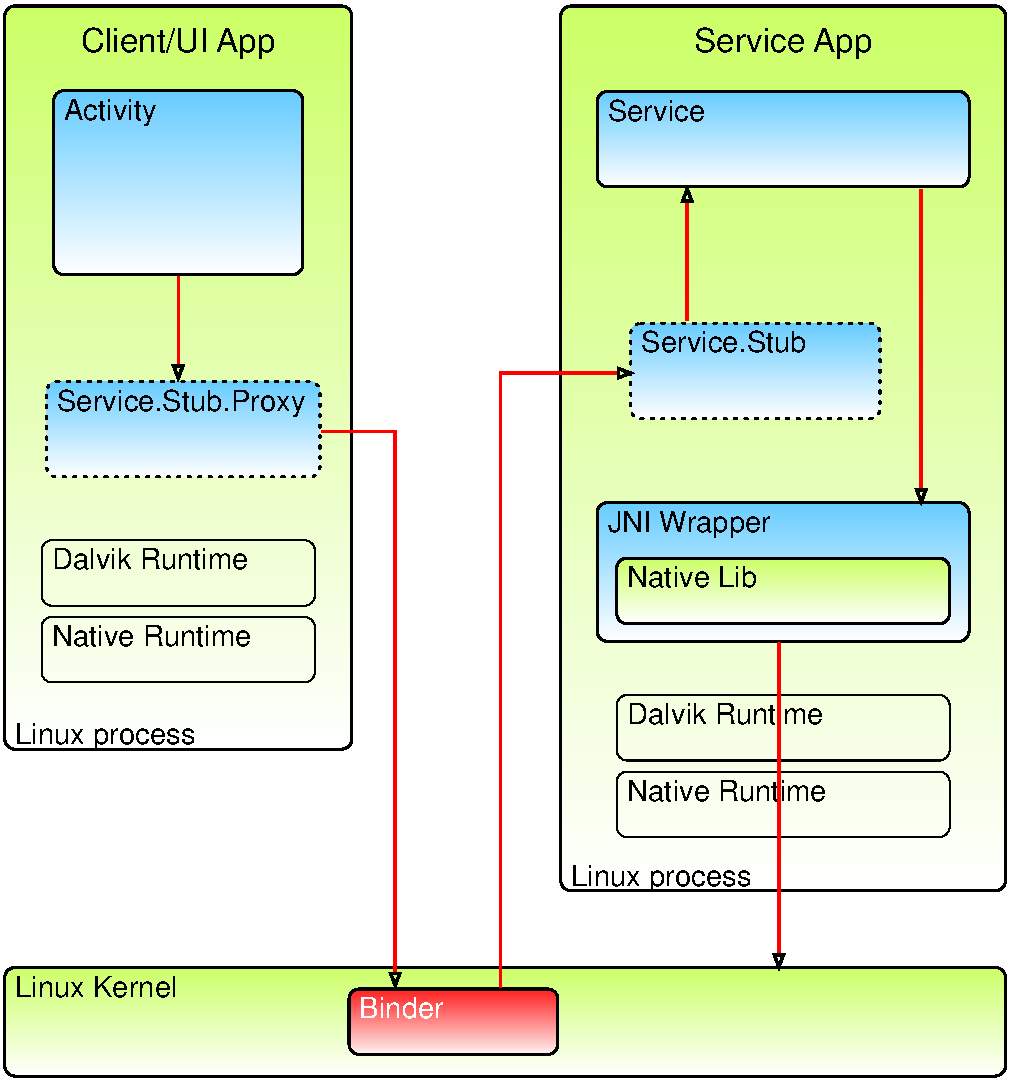
\includegraphics[scale=.4]{images/binder_flow.pdf}
			\caption{Communication Activity-Service through Binder}
			\label{fig:binder_flow}
		\end{figure}
	\item \textsc{Anonymous Shared Memory}\\
	Typically, a first process creates a shared memory region using \textit{ashmem} and uses Binder to share the corresponding file descriptor with other processes with which it wishes to share the region. \textit{Ashmem} destroys memory regions when all processes referring to them have exited and will shrink mapped regions if the system is in need of memory.
	\item \textsc{Alarm}\\
	Android's alarm driver is actually layered on top of the kernel's existing Real-Time Clock (RTC) and High-Resolution Timers (HRT) functionalities. Android's alarm driver cleverly combines the best of both worlds: by default the driver uses the kernel's High-Resolution Timer (HRT) functionality, but whenever the system is about to suspend itself, it programs the RTC so that the system gets woken up at the appropriate time.
	\item \textsc{Logger}\\
	Android defines its own logging mechanisms based on the Android logger driver added to the kernel. The lightweight Android Logger manages a handful of separate kernel-hosted buffers for logging data coming from user-space. The driver maintains circular buffers where it logs every incoming event and returns immediately back to the caller.
	\end{itemize}
So far the most evident kernel customisations have been described, despite they are actually more, nonetheless a deeper analysis of the Android kernel is out of the scope of this document.
\item \textbf{Hardware Abstraction Layer [HAL]}\\
Keeping in mind Fig. \ref{fig:stack}, let's examine the HAL module. The Android stack typically relies on shared libraries provided by manufacturers to interact with hardware. In effect, Android relies on what can be considered a Hardware Abstraction Layer (HAL), and we can mainly identify the following advantages:
	\begin{itemize}
		\item Separates Android platform logic from specific hardware interfaces
		\item User­space HAL offers standard "driver" definitions for graphics, audio, camera, bluetooth, GPS, radio (RIL), WiFi, etc.
		\item Makes porting easier
		\item Other - minor - license-related reasons
	\end{itemize}
\begin{figure}[!htb]
	\centering
	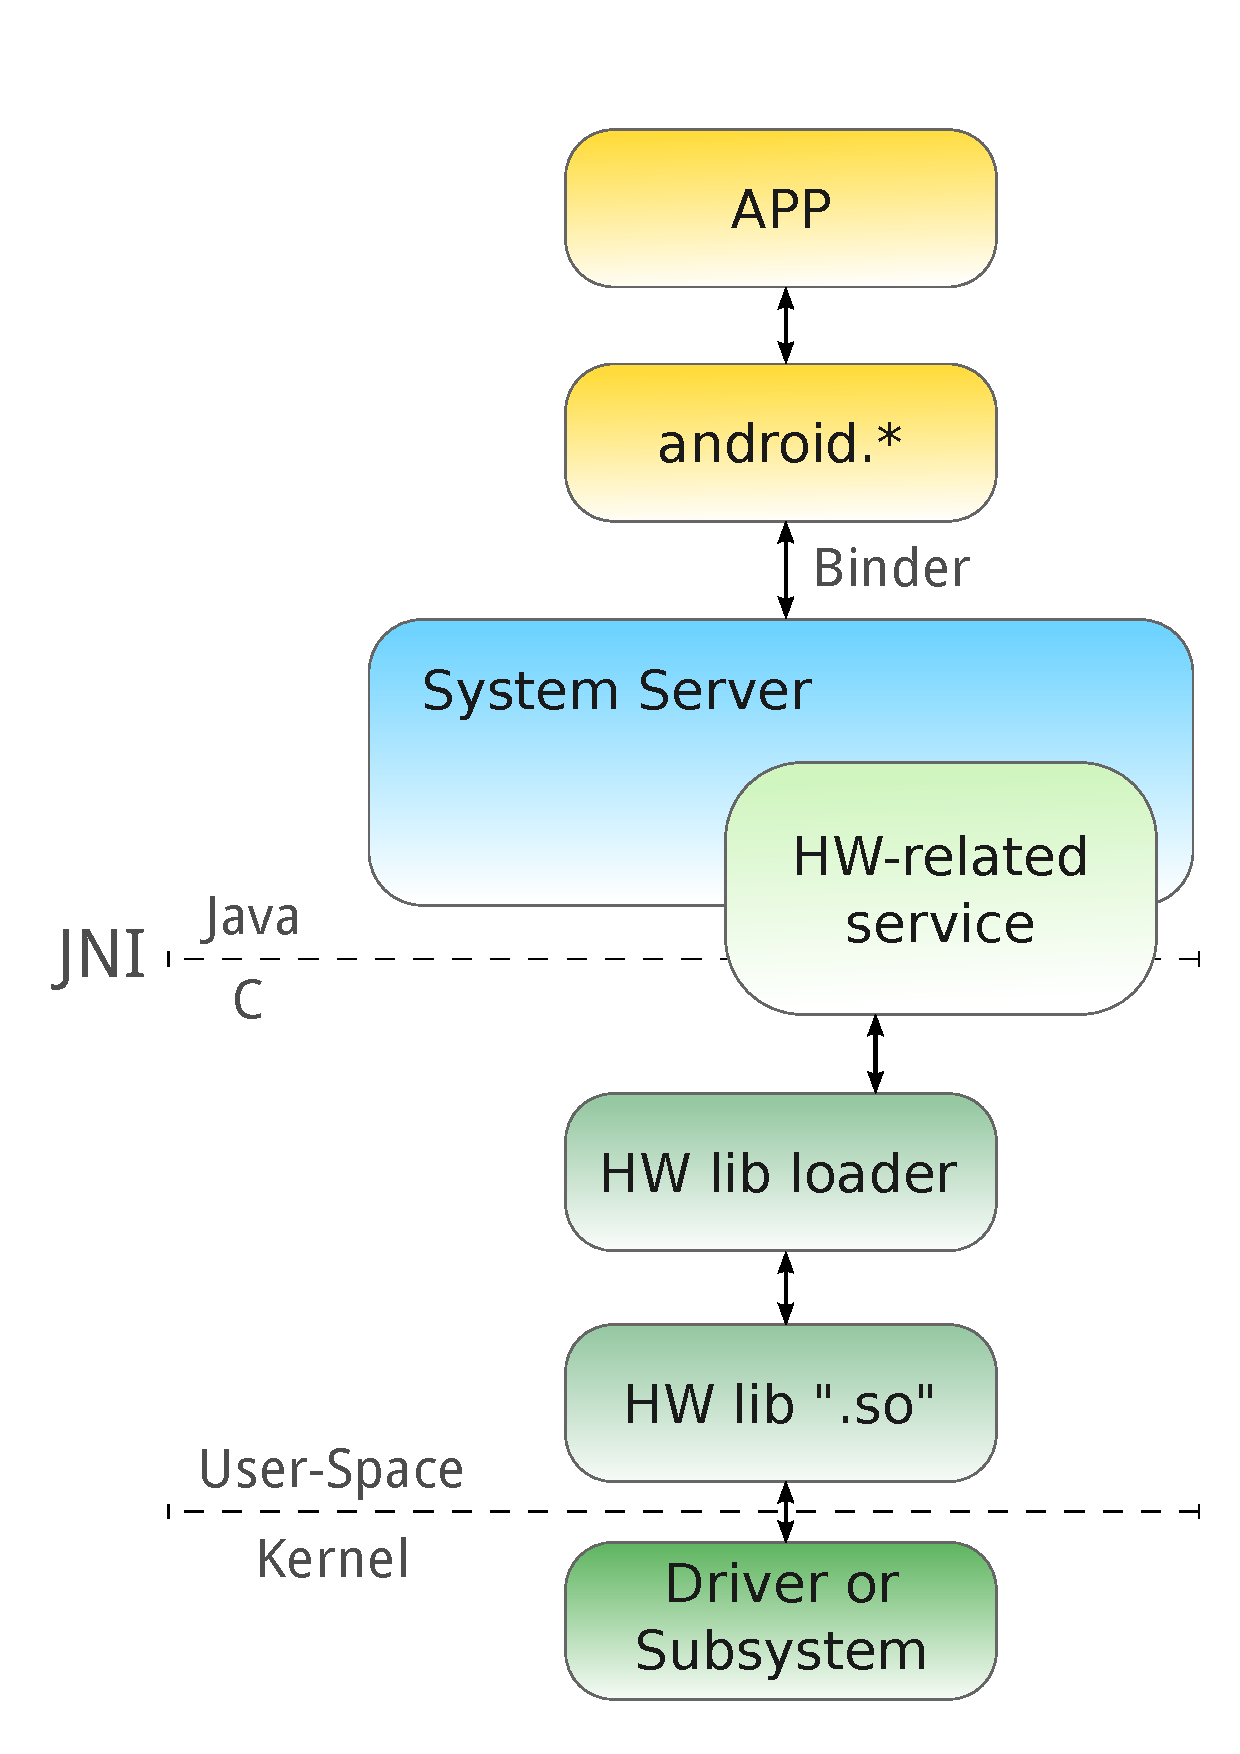
\includegraphics[scale=.25]{images/hal.pdf}
	\caption{Hardware Abstraction Layer structure}
	\label{fig:hal}
\end{figure}
A typical example of the way in which Android abstracts and supports hardware can be seen in Fig. \ref{fig:hal}: it's easy to notice that the hardware support outside the bare Kernel is substantial. As a consequence, Android, to run on a specific hardware, requires more than just a proper driver: a hardware module (not a kernel module) which conforms to the API specified for that type of hardware, must be provided.
\item \textbf{Native Libraries}\\
Android relies on slightly more than a hundred dynamically-loaded libraries (in our testing configuration, 124), which are stored in /system/lib. The largest part of them is actually generated within the AOSP, and a portion comes from external projects, merged into AOSP codebase to add some specific functionalities.
\item \textbf{Native Daemons}\\
As already seen into Linux, Android typically runs some \textit{Daemons}, which are native processes - launched at startup phase, or when expressly requested - that continue to run throughout the lifetime of the system.
\item \textbf{Init}\\
The list of automatically launched daemons during the startup phase (with permission and other options) can be found in \textit{init.rc} file: \textit{\textbf{init}} - as happens into Linux - is the first process started immediately after the Linux boot, and \textit{init.rc} is its configuration file.
\item \textbf{Dalvik VM}\\
Long story short: Dalvik VM is Android's Java Virtual Machine, with a substantial difference, as shown in Fig. \ref{fig:dalvik}, and after written.\\
\begin{figure}[!htb]
	\centering
	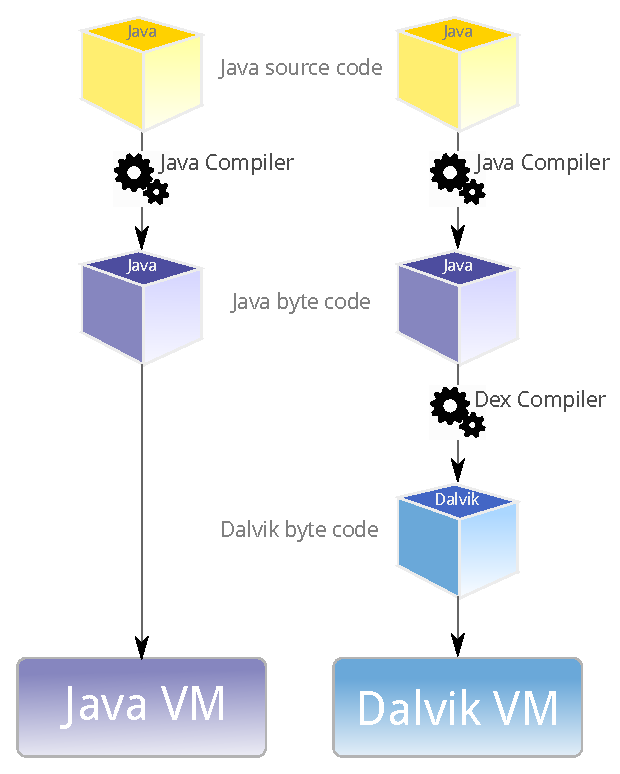
\includegraphics[scale=.7]{images/dalvik.pdf}
	\caption{Comparison Java - Dalvik}
	\label{fig:dalvik}
\end{figure}
While in Java the source code is compiled into Java byte code, which can run on the Java VM, in Android there's one more halfway step, which passes through the \textit{dx utility}, which is a \textit{Dex compiler}: \textit{.dex} files, created by postprocessing the \textit{.class} files generated by the Java compiler - when uncompressed are 50\% smaller than their originating .jar files - can finally run on the Dalvik VM which therefore can't straight run Java byte code.
\definecolor{lightgray}{gray}{0.93}
  \vskip\baselineskip%
  \par\noindent\colorbox{lightgray}{%
    \begin{minipage}{0.953\textwidth}
		\textsc{Good to know}:\\
		In 2010 an interesting feature of Dalvik has been introduced: a Just-In-Time (JIT) compiler for ARM. This compiler allows \textit{.dex} byte code files to be converted to binary assembly instructions that run natively on the target's CPU (only ARM so far) instead of being interpreted one instruction at a time by the VM. The first time you load the app it may take a bit longer, but once an App has been \textit{"JIT-ed"}, then it loads and runs much faster than being interpreted.
    \end{minipage}%
  }%
  \vskip\baselineskip%
\end{itemize}
Before we go on analysing the \textit{System Services} block (again, Fig. \ref{fig:stack}), it's worth focusing on JNI interface, which basically permits the communication between the \textit{Java} world and the \textit{Native} one.
\begin{itemize}
\item \textbf{Java Native Interface [JNI]}\\
Java written code sometimes needs to interface to native code written in C/C++, and this sentence comes especially true in the embedded systems' world: in fact, to access to low-level functionalities, Java applications need to interact with native daemons and libraries. This bridge role is played by what is known as \textit{Java Native Interface}.\\
JNI allows programmers to take advantage of the power of the Java platform, without having to abandon their investments in legacy code: this means also that you can port your C/C++ code to Android with a bit of investment on implementing a sort of \textit{"glue code"} which lets Android applications using it. JNI has been defined as \textit{"a dark art reserved to the initiated"} \cite{embandroid} therefore, for the time being, it's enough to have an idea of what it is.
\item \textbf{System Services}\\
System services (e.g. Location service, Sensor service, WiFi service, Alarm service, Telephony service, Bluetooth service, and so on) are always on, always running, and readily available for developers to tap into, started at boot time and are guaranteed to be running by the time your application launches. They cooperate together through Binder, the mechanism on which all system services are built.\\
System services are basically divided in two parts: mainly Java-coded services (but two), running under the \textit{system server} process, and C/C++ coded services, running under the \textit{media server} process.\\
As we did for JNI, we won't go deeper into the details of System Services now, although we'll better understand its functioning theough an example. Fully understanding the internals of Android's system services has been defined as \textit{trying to swallow a whale} \cite{embandroid}.
\item \textbf{Service Manager}\\
As the director of orchestra, the Service Manager coordinates all the system services, and allows Android Applications to access System Services: as we'll see in the second part of this work, an Application can invoke the
\begin{verbatim}
	serviceManager.getSystemService(SERVICE_NAME);
\end{verbatim} method on the ServiceManager object. This interaction nevertheless isn't as simple as it could seem at first sight, since the whole process uses the Binder paradigm. (Figg. \ref{fig:service_manager} and \ref{fig:binder_flow}) despite Android Development Team made all this quite transparent to the Application developer, who typically doesn't need to implement his own service, but just to use the ones already built by AOSP.
\begin{figure}[!htb]
	\centering
	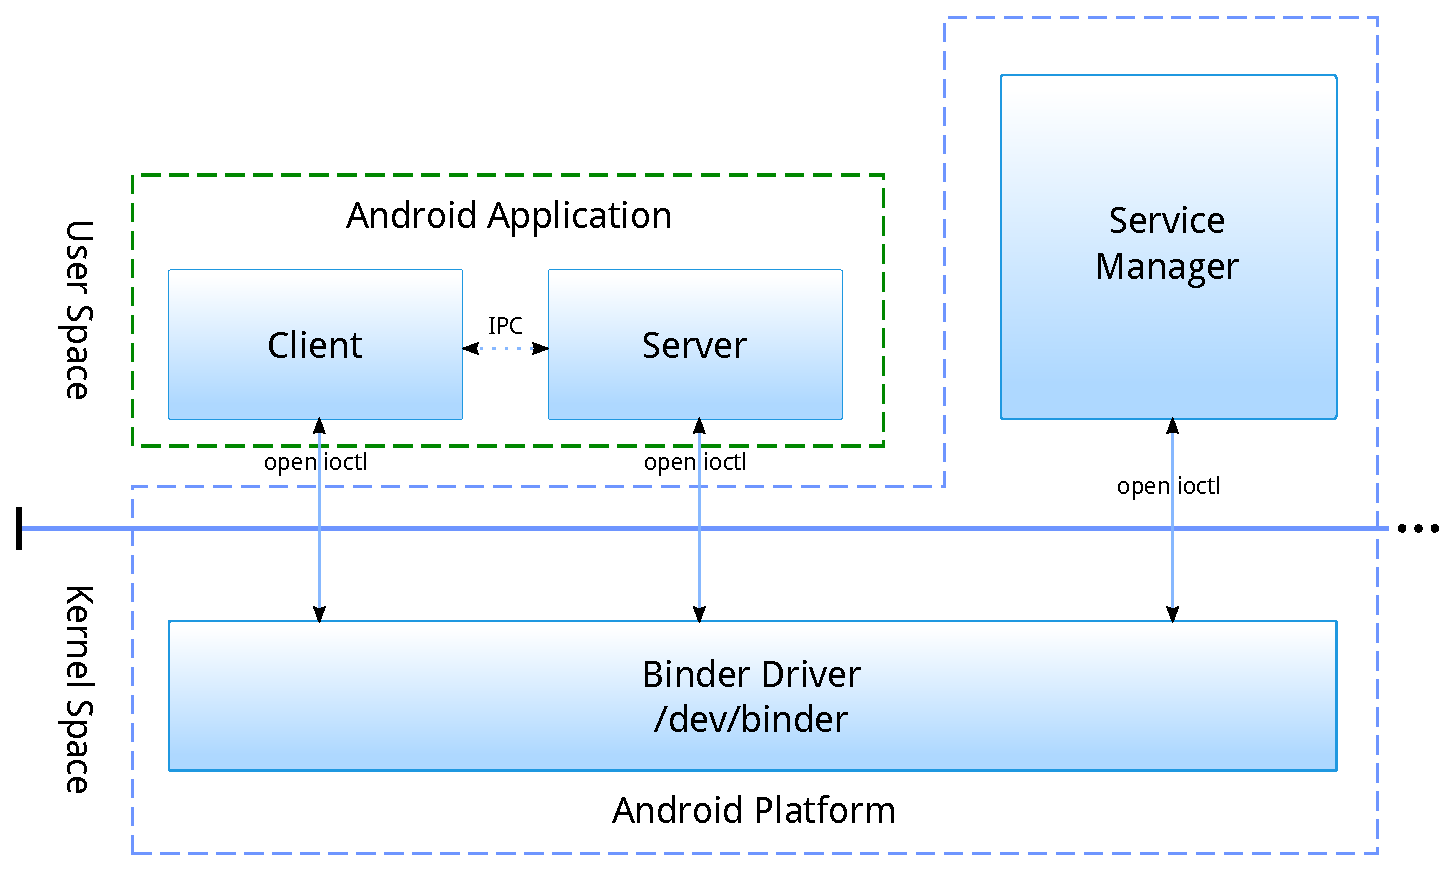
\includegraphics[scale=.5]{images/service_manager.pdf}
	\caption{Interaction "Application - Service manager", through Binder}
	\label{fig:service_manager}
\end{figure}
\item \textbf{Android Framework Libraries}\\
Libraries that allow the Application, through Java Interfaces, to access the proper native libraries: whenever an instance of a library class is created, a call to the ServiceManager - through binder - is made, to get the proper Service (or System Service) as Interface (binded to an .aidl file), which finally permits the Application to call Java libraries' methods that, through JNI, are connected to the native library.
\end{itemize}
The higher level isn't that much of our interest for this work, as it includes the "Apps" layer, which actually are called "Activities", and they are just the presentation level of the whole stack. Nevertheless we will see in the last part of this work (Section \ref{Customising}.) the implementation of a very simple Activity to graphically interact with our custom native daemon.